\documentclass[11pt,a4paper]{scrartcl}
\usepackage[czech]{babel}
\usepackage[utf8]{inputenc}
\usepackage{graphicx}
\usepackage{float}
\graphicspath{{./img/}}

\begin{document}
	\begin{figure}[h!]
		\centering
		
\includegraphics[bb= 0 0 820 445 , width=75mm]{favlogo.jpg}
	\end{figure}
	
	\vspace{5cm}
	
	{\centering
		{\huge KIV/OS - Semestrální práce}\\[1em]
		{\large Simulátor operačního systému}\\[7,5cm]
	}
	
	\begin{center}
		\begin{tabular}{l r}
		student: & Daniel HRYZBIL, Anežka JÁCHYMOVÁ, Zdeněk VALEŠ\\
		datum: & 29.11.2019\\
		\end{tabular}
	\end{center}
	
	\thispagestyle{empty}
	\newpage
	
	\section{Zadání}
	\begin{enumerate}
		\item 	Vytvořte virtuální stroj, který bude simulovat OS
		\item 	Součástí bude shell s gramatikou cmd, tj. včetně exit
		\item 	Vytvoříte ekvivalenty standardních příkazů a programů:
		\begin{enumerate}
			\item echo, cd, dir, md, rd, type, find /v /c"" (tj. co dělá wc v unix-like prostředí), sort, tasklist, shutdown
			
			\begin{enumerate}
				\item	cd musí umět relativní cesty
				\item	echo musí umět @echo on a off
				\item	type musí umět vypsat jak stdin, tak musí umět vypsat soubor
			\end{enumerate}
		
			\item	Dále vytvoříte programy rgen a freq
			\item	rgen bude vypisovat náhodně vygenerovaná čísla v plovoucí čárce na stdout, dokud mu nepřijde znak Ctrl+Z //EOF
			\item	freq bude číst z stdin a sestaví frekvenční tabulku bytů, kterou pak vypíše pro všechny byty s frekvencí větší než 0 ve formátu: “0x\%hhx : \%d”
		\end{enumerate}
		\item 	Implementujte roury a přesměrování
		\item 	Nebudete přistupovat na souborový systém, ale použijete simulovaný disk
		
		\begin{enumerate}
			\item 	Za 5 bonusových bodů můžete k realizaci souborového systému použít semestrální práci z KIV/ZOS - tj. implementace FAT.
		\end{enumerate}
	\end{enumerate}

	\section{Kernel}
	Jádro poskytuje API pro správu procesů a vláken, vytvoření pipe a přístup k disku. TODO: trochu rozvést
	
	Základním konceptem kernelu je třída \verb|HandleStorage| společně s \verb|HandleReference|. Každá třída reprezentující nějaký handle (soubor, proces, vlákno, ...) implementuje rozhraní \verb|IHandle|. Všechny instance těchto tříd jsou následně uloženy uvnitř \verb|HandleStorage|, kde jim je přiřazeno jejich unikátní \verb|HandleID| (16 bitové číslo). Přístup k uloženým handle je následně možný pouze přes objekty \verb|HandleReference|. Struktura handlerů je znázorněna diagramem tříd na obrázku \ref{fig:handle-class-d}.
	
	\begin{figure}[H]
		\centering
		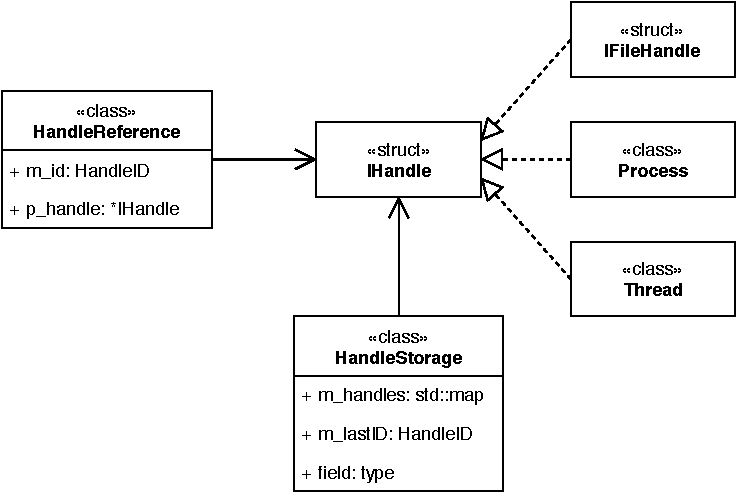
\includegraphics[width=11cm]{handle-class-d.pdf}
		\caption{Diagram tříd handlerů}
		\label{fig:handle-class-d}
	\end{figure}
	
	Uvnitř \verb|HandleStorage| je pro každý handle uložený počet referencí na tento handle, který se inkrementuje vždy při vytvoření nové \verb|HandleReference| a dekrementuje při odstranění \verb|HandleReference|. Handly s nulovým počtem referencí jsou automaticky uzavřeny a odstraněny ze systému. 
	
	Každý proces si udržuje vlastní množinu referencí na handly, které byly v jeho kontextu vytvořeny nebo jinak získány (například při vytváření procesu předá rodičovský proces nově vytvořenému procesu handle na \verb|stdin| a \verb|stdout|). Tato množina se zároveň používá i pro zjištění, zda má proces k nějakému handlu vůbec přístup. Při odstranění nějakého procesu potom dojde k odstranění všech handle referencí uložených v jeho množině, a tím dojde automaticky i k odstranění všech handlů, které používal pouze daný proces. 
	
	Kernel se tak nespoléhá na "slušnost" user-space kódu, který by měl vždy použít \verb|CloseHandle|, ale dokáže při ukončení procesu automaticky uklidit všechny nepotřebné handly, stejně jako reálný OS. Zároveň tento koncept umožňuje i efektivnější spolupráci více vláken najednou. Při práci s nějakým handle totiž není potřeba zamykat globální zámky, protože pokud pro tento handle existuje alespoň jeden objekt \verb|HandleReference|, tak je zaručeno, že žádné jiné vlákno nemůže tento handle nečekaně odstranit a způsobit tak pád celého systému.
	
	\subsection{Procesy a vlákna}
	
	Procesy jsou uloženy v již zmíněném \verb|HandleStorage| a \verb|HandleID| je bráno jako PID. Stejně tak jsou uložena i vlákna a \verb|HandleID| představuje TID.
	
	Každé vlákno simulovaného OS využívá reálné vlákno fyzického OS (\verb|std::thread|). Kernel dále neobsahuje žádný platform-specific kód, kromě načítání "user.dll". Za hlavní vlákno procesu se považuje jeho první vlákno. Při vytvoření procesu je vždy vytvořeno i jeho hlavní vlákno.
	
	\subsubsection{API}
	\begin{itemize}
		\item CreateProcess
		\item Clone
		\item CreateThread
		\item WaitFor
		\item GetExitCode
		\item Exit
		\item SetupSignal
		\item SystemShutdown	
	\end{itemize}
	
	\subsection{Filesystem}
	
	Kernel obsahuje file system manager, který spravuje disky a souborové systémy na nich uložené. Pro přístup na disk je použito abstraktní API, které každý ovladač pro FS. Struktura je znázorněna na obrázku \ref{fig:fs-layers}. Jako filesystem jsme zvolili FAT implementovanou v rámci KIV/ZOS.
	
	\begin{figure}[H]
		\centering
		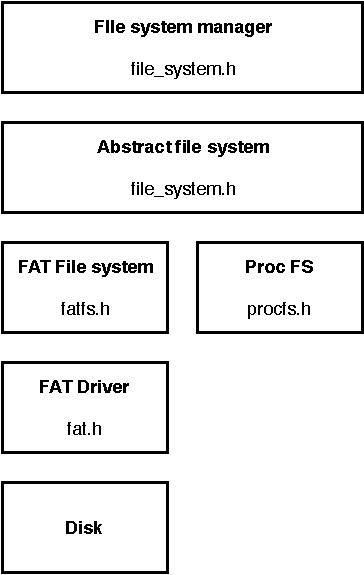
\includegraphics[height=9cm]{fs-layers.pdf}
		\caption{Struktura správy souborového systému}
		\label{fig:fs-layers}
	\end{figure}
	
	\begin{figure}[H]
		\centering
		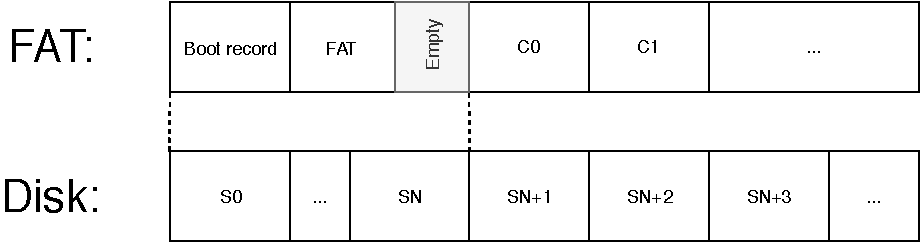
\includegraphics[width=12cm]{fat-rozdeleni-disku.pdf}
		\caption{Uložení FAT souborového systému na disk}
		\label{fig:fat-disk-struct}
	\end{figure}

	\subsubsection{ProcFS}
	Na virtuálním disku 0. Používá se k získání právě běžících procesů.
	
	\subsubsection{API}
	\begin{itemize}
		\item Create
		\item Query
		\item Read
		\item ReadDir
		\item Remove
		\item Resize
		\item Write
	\end{itemize}

	
	\subsection{Pipe}
	
	Pipe je vytvořena dvěma handly - \verb|PipeReadEnd| a \verb|PipeWriteEnd|. Viz obrázek \ref{fig:pipe-c}.
	
	\begin{figure}[H]
		\centering
		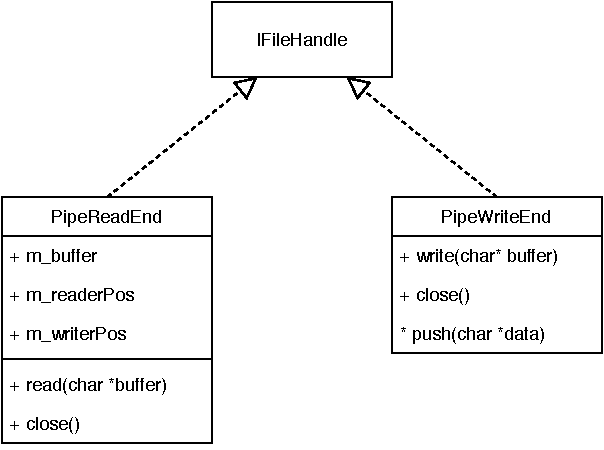
\includegraphics[width=8cm]{pipe-c.pdf}
		\caption{Pipe diagram tříd}
		\label{fig:pipe-c}
	\end{figure}
	
	\section{RTL}
	
	\section{Shell a uživatelské příkazy}
	
	\section{Závěr}
	
\end{document}
